% Options for packages loaded elsewhere
\PassOptionsToPackage{unicode}{hyperref}
\PassOptionsToPackage{hyphens}{url}
\PassOptionsToPackage{dvipsnames,svgnames,x11names}{xcolor}
%
\documentclass[
  11pt,
  a4paper,
]{article}

\usepackage{amsmath,amssymb}
\usepackage{setspace}
\usepackage{iftex}
\ifPDFTeX
  \usepackage[T1]{fontenc}
  \usepackage[utf8]{inputenc}
  \usepackage{textcomp} % provide euro and other symbols
\else % if luatex or xetex
  \usepackage{unicode-math}
  \defaultfontfeatures{Scale=MatchLowercase}
  \defaultfontfeatures[\rmfamily]{Ligatures=TeX,Scale=1}
\fi
\usepackage{lmodern}
\ifPDFTeX\else  
    % xetex/luatex font selection
  \setmainfont[]{Times New Roman}
  \setsansfont[]{Helvetica}
  \setmonofont[]{Courier New}
\fi
% Use upquote if available, for straight quotes in verbatim environments
\IfFileExists{upquote.sty}{\usepackage{upquote}}{}
\IfFileExists{microtype.sty}{% use microtype if available
  \usepackage[]{microtype}
  \UseMicrotypeSet[protrusion]{basicmath} % disable protrusion for tt fonts
}{}
\makeatletter
\@ifundefined{KOMAClassName}{% if non-KOMA class
  \IfFileExists{parskip.sty}{%
    \usepackage{parskip}
  }{% else
    \setlength{\parindent}{0pt}
    \setlength{\parskip}{6pt plus 2pt minus 1pt}}
}{% if KOMA class
  \KOMAoptions{parskip=half}}
\makeatother
\usepackage{xcolor}
\usepackage[lmargin=25mm,rmargin=25mm,tmargin=25mm,bmargin=25mm]{geometry}
\setlength{\emergencystretch}{3em} % prevent overfull lines
\setcounter{secnumdepth}{-\maxdimen} % remove section numbering
% Make \paragraph and \subparagraph free-standing
\ifx\paragraph\undefined\else
  \let\oldparagraph\paragraph
  \renewcommand{\paragraph}[1]{\oldparagraph{#1}\mbox{}}
\fi
\ifx\subparagraph\undefined\else
  \let\oldsubparagraph\subparagraph
  \renewcommand{\subparagraph}[1]{\oldsubparagraph{#1}\mbox{}}
\fi


\providecommand{\tightlist}{%
  \setlength{\itemsep}{0pt}\setlength{\parskip}{0pt}}\usepackage{longtable,booktabs,array}
\usepackage{calc} % for calculating minipage widths
% Correct order of tables after \paragraph or \subparagraph
\usepackage{etoolbox}
\makeatletter
\patchcmd\longtable{\par}{\if@noskipsec\mbox{}\fi\par}{}{}
\makeatother
% Allow footnotes in longtable head/foot
\IfFileExists{footnotehyper.sty}{\usepackage{footnotehyper}}{\usepackage{footnote}}
\makesavenoteenv{longtable}
\usepackage{graphicx}
\makeatletter
\def\maxwidth{\ifdim\Gin@nat@width>\linewidth\linewidth\else\Gin@nat@width\fi}
\def\maxheight{\ifdim\Gin@nat@height>\textheight\textheight\else\Gin@nat@height\fi}
\makeatother
% Scale images if necessary, so that they will not overflow the page
% margins by default, and it is still possible to overwrite the defaults
% using explicit options in \includegraphics[width, height, ...]{}
\setkeys{Gin}{width=\maxwidth,height=\maxheight,keepaspectratio}
% Set default figure placement to htbp
\makeatletter
\def\fps@figure{htbp}
\makeatother

\definecolor{darkblue}{RGB}{0,70,140}
\makeatletter
\makeatother
\makeatletter
\makeatother
\makeatletter
\@ifpackageloaded{caption}{}{\usepackage{caption}}
\AtBeginDocument{%
\ifdefined\contentsname
  \renewcommand*\contentsname{Table of contents}
\else
  \newcommand\contentsname{Table of contents}
\fi
\ifdefined\listfigurename
  \renewcommand*\listfigurename{List of Figures}
\else
  \newcommand\listfigurename{List of Figures}
\fi
\ifdefined\listtablename
  \renewcommand*\listtablename{List of Tables}
\else
  \newcommand\listtablename{List of Tables}
\fi
\ifdefined\figurename
  \renewcommand*\figurename{Figure}
\else
  \newcommand\figurename{Figure}
\fi
\ifdefined\tablename
  \renewcommand*\tablename{Table}
\else
  \newcommand\tablename{Table}
\fi
}
\@ifpackageloaded{float}{}{\usepackage{float}}
\floatstyle{ruled}
\@ifundefined{c@chapter}{\newfloat{codelisting}{h}{lop}}{\newfloat{codelisting}{h}{lop}[chapter]}
\floatname{codelisting}{Listing}
\newcommand*\listoflistings{\listof{codelisting}{List of Listings}}
\makeatother
\makeatletter
\@ifpackageloaded{caption}{}{\usepackage{caption}}
\@ifpackageloaded{subcaption}{}{\usepackage{subcaption}}
\makeatother
\makeatletter
\@ifpackageloaded{tcolorbox}{}{\usepackage[skins,breakable]{tcolorbox}}
\makeatother
\makeatletter
\@ifundefined{shadecolor}{\definecolor{shadecolor}{rgb}{.97, .97, .97}}
\makeatother
\makeatletter
\makeatother
\makeatletter
\makeatother
\ifLuaTeX
  \usepackage{selnolig}  % disable illegal ligatures
\fi
\IfFileExists{bookmark.sty}{\usepackage{bookmark}}{\usepackage{hyperref}}
\IfFileExists{xurl.sty}{\usepackage{xurl}}{} % add URL line breaks if available
\urlstyle{same} % disable monospaced font for URLs
\hypersetup{
  pdftitle={MAST32001 Computational Statistics},
  pdfauthor={Kaiwei Fu; Lingyu Wang; Sami Sönkä; Zhi Zhou},
  colorlinks=true,
  linkcolor={darkblue},
  filecolor={Maroon},
  citecolor={darkblue},
  urlcolor={darkblue},
  pdfcreator={LaTeX via pandoc}}

\title{MAST32001 Computational Statistics}
\usepackage{etoolbox}
\makeatletter
\providecommand{\subtitle}[1]{% add subtitle to \maketitle
  \apptocmd{\@title}{\par {\large #1 \par}}{}{}
}
\makeatother
\subtitle{Course Final Assignment, WS 2026}
\author{Kaiwei Fu \and Lingyu Wang \and Sami Sönkä \and Zhi Zhou}
\date{2026-10-23}

\begin{document}
\maketitle
\ifdefined\Shaded\renewenvironment{Shaded}{\begin{tcolorbox}[interior hidden, boxrule=0pt, frame hidden, enhanced, borderline west={3pt}{0pt}{shadecolor}, breakable, sharp corners]}{\end{tcolorbox}}\fi

\setstretch{1.25}
\hypertarget{task-1-time-series-bootstrap-and-the-ladle-estimator}{%
\section{Task 1: Time series bootstrap and the ladle
estimator}\label{task-1-time-series-bootstrap-and-the-ladle-estimator}}

\hypertarget{part-a-whitening-and-autocovariance-matrices}{%
\subsection{Part A: Whitening and autocovariance
matrices}\label{part-a-whitening-and-autocovariance-matrices}}

\hypertarget{conventions-and-implementation}{%
\subsubsection{Conventions and
implementation}\label{conventions-and-implementation}}

The observations are stored as the rows of an \(n\times p\) matrix
\(X\). Each variable is centred using its full-sample column mean,

\[
X_c=X-\mathbf{1}_n\bar{x}^{\mathsf T},
\qquad
S_0=\frac{1}{n-1}X_c^{\mathsf T}X_c.
\]

If \(S_0=VDV^{\mathsf T}\), the symmetric whitening matrix and whitened
data are

\[
W=S_0^{-1/2}=VD^{-1/2}V^{\mathsf T},
\qquad Y=X_cW.
\]

Eigenvalues below \(10^{-10}\) times the largest eigenvalue are treated
as numerically zero because their inverse square roots would be
unstable. No additional marginal scaling is applied because scaling is
already included in \(W\).

For lag \(h\geq1\), we estimate

\[
\widehat C_h
=\frac{1}{n-h}\sum_{t=1}^{n-h}y_ty_{t+h}^{\mathsf T}.
\]

The mean is not re-estimated within each lag window. Row \(t\) is paired
with row \(t+h\), and normalization uses the \(n-h\) available pairs.
The matrices used for joint diagonalization are symmetrized as
\(\widehat C_h^{(s)}=(\widehat C_h+\widehat C_h^{\mathsf T})/2\).

\hypertarget{purpose-and-numerical-verification}{%
\subsubsection{Purpose and numerical
verification}\label{purpose-and-numerical-verification}}

Whitening removes contemporaneous scale and cross-covariance, so the
lag-zero sample covariance becomes \(I_p\). In the second-order
source-separation model, this changes the unknown mixing matrix into an
orthogonal matrix, allowing the remaining directions to be estimated by
orthogonal joint diagonalization. Whitening does not make the
observations serially independent; non-zero-lag dependence remains in
the autocovariance matrices and provides the information used to
identify the signal directions.

For the supplied data, \(n=1000\) and \(p=10\). The numerical checks
gave

\[
\max_j|\bar y_j|=6.49\times10^{-14},\qquad
\max_{j,k}\left|\left\{\widehat{\operatorname{Cov}}(Y)-I_{10}\right\}_{jk}\right|
=3.55\times10^{-15}.
\]

The whitened variances ranged from \(0.999999999999997\) to \(1\), and
the largest absolute off-diagonal covariance was \(2.58\times10^{-15}\).
These values confirm the expected whitening effect to numerical
precision. The non-zero Frobenius norms of the lagged matrices,
including \(0.3653\) at lag 1 and \(0.5575\) at lag 2, also show that
whitening does not force non-zero-lag covariance estimates to zero.

\begin{figure}

{\centering \includegraphics[width=0.88\textwidth,height=\textheight]{output/figures/task1_whitening_covariance.png}

}

\caption{\label{fig-task1-whitening}Original contemporaneous correlation
and covariance after whitening.}

\end{figure}

\hypertarget{part-b-bootstrap-for-dependent-observations}{%
\subsection{Part B: Bootstrap for dependent
observations}\label{part-b-bootstrap-for-dependent-observations}}

\hypertarget{fixed-block-bootstrap}{%
\subsubsection{Fixed-block bootstrap}\label{fixed-block-bootstrap}}

For block length \(L\), a starting position is sampled uniformly with
replacement from \(\{1,\ldots,n-L+1\}\). The corresponding \(L\)
consecutive multivariate rows are retained in their original order. This
is repeated \(\lceil n/L\rceil\) times, after which the blocks are
concatenated and truncated to \(n\) rows. The tuning parameter \(L\)
determines how much local dependence can be retained within each block.

\hypertarget{stationary-bootstrap}{%
\subsubsection{Stationary bootstrap}\label{stationary-bootstrap}}

The stationary bootstrap begins at an index sampled uniformly from
\(\{1,\ldots,n\}\). At every subsequent position, a new uniform index is
selected with probability \(r=1/L\); otherwise, the previous index is
advanced by one, with circular wrap-around from \(n\) to 1.
Consequently, each block length \(K\) has the geometric distribution

\[
\Pr(K=k)=r(1-r)^{k-1},\qquad E(K)=\frac{1}{r}=L.
\]

Unlike the fixed-block method, the stationary bootstrap uses random
block lengths. In 100 generated samples, target expected lengths 10, 20
and 40 gave mean observed lengths 9.94, 20.20 and 40.94, respectively.

\hypertarget{why-iid-resampling-is-unsuitable}{%
\subsubsection{Why IID resampling is
unsuitable}\label{why-iid-resampling-is-unsuitable}}

Resampling individual rows independently destroys temporal ordering and
makes non-zero-lag autocovariances approximately zero. Such samples do
not represent the variability of statistics calculated from the original
dependent process. Both block procedures instead resample consecutive
multivariate observations, preserving local serial and cross-series
dependence within blocks.

\begin{figure}

{\centering \includegraphics[width=0.78\textwidth,height=\textheight]{output/figures/task1_bootstrap_acf_comparison.png}

}

\caption{\label{fig-task1-acf-comparison}Example ACF comparison for the
variable with the largest absolute lag-1 sample ACF.}

\end{figure}

\hypertarget{effect-of-block-length}{%
\subsubsection{Effect of block length}\label{effect-of-block-length}}

Dependence preservation was evaluated using the mean absolute difference
between the original and bootstrap sample autocorrelations, averaged
over all 10 variables and lags 1--20. Each row of
Table~\ref{tbl-task1-acf-error} summarizes 100 bootstrap samples.

\hypertarget{tbl-task1-acf-error}{}
\begin{longtable}[]{@{}lrr@{}}
\caption{\label{tbl-task1-acf-error}Mean absolute ACF error; smaller
values indicate better local-dependence preservation.}\tabularnewline
\toprule\noalign{}
Method & Mean error & Standard deviation \\
\midrule\noalign{}
\endfirsthead
\toprule\noalign{}
Method & Mean error & Standard deviation \\
\midrule\noalign{}
\endhead
\bottomrule\noalign{}
\endlastfoot
IID & 0.0460 & 0.0017 \\
Fixed, \(L=10\) & 0.0381 & 0.0021 \\
Fixed, \(L=20\) & 0.0320 & 0.0019 \\
Fixed, \(L=40\) & 0.0270 & 0.0025 \\
Stationary, \(E(K)=10\) & 0.0336 & 0.0020 \\
Stationary, \(E(K)=20\) & 0.0295 & 0.0024 \\
Stationary, \(E(K)=40\) & 0.0269 & 0.0027 \\
\end{longtable}

IID resampling has the largest error. Longer blocks preserve the
observed ACF more closely, although they provide fewer effectively
independent blocks and slightly greater Monte Carlo variability. Block
length is therefore a tuning choice that balances dependence
preservation against the number of resampled blocks.

\begin{figure}

{\centering \includegraphics[width=0.9\textwidth,height=\textheight]{output/figures/task1_bootstrap_acf_error.png}

}

\caption{\label{fig-task1-acf-error}Distribution of ACF error over 100
bootstrap samples for each method and block length.}

\end{figure}

\hypertarget{part-c-the-ladle-quantities}{%
\subsection{Part C: The ladle
quantities}\label{part-c-the-ladle-quantities}}

\hypertarget{eigenvalue-based-quantity-phi}{%
\subsubsection{\texorpdfstring{Eigenvalue-based quantity
\(\phi\)}{Eigenvalue-based quantity \textbackslash phi}}\label{eigenvalue-based-quantity-phi}}

For the lag set \(\mathcal T\), an orthogonal matrix \(U\) approximately
jointly diagonalizes the whitened autocovariance matrices. The component
strengths are

\[
s_j=\sum_{h\in\mathcal T}
\left[
\operatorname{diag}\!\left(U^{\mathsf T}\widehat C_h^{(s)}U\right)_j
\right]^2,
\]

ordered so that \(s_0\geq\cdots\geq s_{p-1}\). The normalized scree
contribution is

\[
\phi(k)=\frac{s_k}{1+\sum_{\ell=0}^{p-1}s_\ell},
\qquad k=0,\ldots,p-1.
\]

Large values correspond to directions with serial dependence, while
noise directions should have strengths close to zero. When several lags
are used, \(U\) is obtained with \texttt{JADE::rjd}; the strength
calculation and ordering are implemented directly.

\hypertarget{bootstrap-variability-quantity-f}{%
\subsubsection{\texorpdfstring{Bootstrap-variability quantity
\(f\)}{Bootstrap-variability quantity f}}\label{bootstrap-variability-quantity-f}}

Let \(\widehat B_k\) and \(B^*_{k,b}\) contain the first \(k\) ordered
directions from the original sample and bootstrap sample \(b\). Their
subspace instability is measured by

\[
f_0(k)=\frac{1}{B}\sum_{b=1}^{B}
\left\{1-\left|\det\!\left(\widehat B_k^{\mathsf T}B^*_{k,b}\right)\right|\right\},
\quad k=1,\ldots,p-1,
\qquad f_0(0)=0,
\]

and normalized as

\[
f(k)=\frac{f_0(k)}{1+\sum_{\ell=0}^{p-1}f_0(\ell)}.
\]

The absolute determinant measures agreement between the two
\(k\)-dimensional subspaces and is invariant to sign changes of
individual directions. Stable signal subspaces have small \(f(k)\),
while variability increases when noise directions enter the estimated
subspace.

\hypertarget{combination-and-dimension-estimate}{%
\subsubsection{Combination and dimension
estimate}\label{combination-and-dimension-estimate}}

The ladle criterion combines the two sources of information:

\[
g(k)=f(k)+\phi(k),\qquad
\widehat q=\underset{k\in\{0,\ldots,p-1\}}{\arg\min}\;g(k).
\]

The scree contribution decreases as weak or noise directions are
included, whereas the bootstrap contribution increases when the
estimated subspace becomes unstable. Their sum balances signal strength
and subspace stability.

\hypertarget{simulation-check}{%
\subsubsection{Simulation check}\label{simulation-check}}

The implementation was checked using Setting 1 of Nordhausen and Virta:
five Gaussian AR/MA signal series and five Gaussian white-noise series,
giving \(p=10\) and true dimension \(q=5\). The check used \(n=1000\),
lags 1--12, 100 bootstrap samples and block length 20. Both the
fixed-block and stationary bootstrap versions returned \(\widehat q=5\).

The largest whitening identity error was \(3.22\times10^{-15}\), the
largest orthogonality error in \(U^{\mathsf T}U\) was
\(2.22\times10^{-15}\), and the joint off-diagonal squared-energy ratio
was \(0.0718\). These checks verify the whitening, orthogonal
directions, approximate joint diagonalization and recovery of the known
signal dimension.

\begin{figure}

{\centering \includegraphics[width=0.92\textwidth,height=\textheight]{output/figures/task1_ladle_criterion.png}

}

\caption{\label{fig-task1-ladle}The implemented \(f\), \(\phi\) and
\(g\) on Setting 1 data. Both bootstrap versions attain their minimum at
the true dimension \(q=5\).}

\end{figure}

\hypertarget{part-d-simulation-study}{%
\subsection{Part D: Simulation study}\label{part-d-simulation-study}}

\hypertarget{simulation-setting-and-study-design}{%
\subsubsection{Simulation setting and study
design}\label{simulation-setting-and-study-design}}

The purpose of the simulation is to assess whether the implementation
recovers a known signal dimension, and how its performance changes with
sample size, bootstrap method and block length. We use Setting 1 of
Nordhausen and Virta, with \(p=10\) components and true signal dimension
\(q=5\). The model has identity mixing, \(x_t=z_t\), where the first
five components are independent Gaussian AR/MA processes and the
remaining five are independent Gaussian white-noise series. The signal
parameters are listed in Table~\ref{tbl-de-processes}, using the
convention

\[
z_{j,t}=\sum_{\ell=1}^{r_j}a_{j,\ell}z_{j,t-\ell}
      +\varepsilon_{j,t}
      +\sum_{\ell=1}^{s_j}b_{j,\ell}\varepsilon_{j,t-\ell},
\qquad \varepsilon_{j,t}\overset{\mathrm{iid}}{\sim}N(0,1).
\]

Innovations are independent across components. The five noise series
also have independent \(N(0,1)\) observations. As in the implementation
used in Part C, each generated column is centred and scaled to unit
sample variance before the whitening step.

\hypertarget{tbl-de-processes}{}
\begin{longtable}[]{@{}cll@{}}
\caption{\label{tbl-de-processes}Signal processes in Setting 1. A dash
denotes an absent AR or MA part.}\tabularnewline
\toprule\noalign{}
Component & AR coefficients & MA coefficients \\
\midrule\noalign{}
\endfirsthead
\toprule\noalign{}
Component & AR coefficients & MA coefficients \\
\midrule\noalign{}
\endhead
\bottomrule\noalign{}
\endlastfoot
1 & \((0.6)\) & \((0,-0.4)\) \\
2 & \((0.4,0.1,0.3)\) & \((0.2,0.4)\) \\
3 & \((0.4)\) & -- \\
4 & -- & \((0.5,0.3,0.1,0.2)\) \\
5 & \((0.1,0.1,0.3)\) & -- \\
\end{longtable}

We consider \(n\in\{200,500,1000\}\), the SOBI lag set
\(\mathcal T=\{1,\ldots,12\}\), and both fixed-block and stationary
bootstrap methods. For each method, \(L\in\{10,20,40\}\) denotes the
fixed or expected block length, respectively. These choices match the
corresponding settings in the paper. This study focuses on SOBI,
extending the implementation from Parts A--C; it does not repeat the
paper's separate AMUSE comparison.

For each sample size, \(R=100\) independent datasets are generated. Each
dataset is analysed under all six method--length combinations, giving
\(1800\) ladle fits. Each fit uses \(B=100\) bootstrap samples. The
paper uses \(2000\) simulation repetitions and \(200\) bootstrap samples
per fit; our smaller experiment is intended to reproduce the main
qualitative behaviour while keeping the computational cost manageable.
Here \(R\) measures variation between independently generated datasets,
whereas \(B\) controls the Monte Carlo approximation within a single
ladle fit.

\hypertarget{computational-procedure-and-tuning-choices}{%
\subsubsection{Computational procedure and tuning
choices}\label{computational-procedure-and-tuning-choices}}

For each generated dataset, the calculation proceeds as follows.

\begin{enumerate}
\def\labelenumi{\arabic{enumi}.}
\item
  Centre the observations and whiten them using the symmetric inverse
  square root of the sample covariance matrix, following the conventions
  in Part A. Compute the symmetrized autocovariance matrices at lags
  \(1,\ldots,12\).
\item
  Apply \texttt{JADE::rjd} to obtain the orthogonal joint diagonalizer.
  Order its directions by decreasing sums of squared diagonal
  autocovariances. These strengths determine the scree contribution
  \(\phi(k)\) from Part C.
\item
  Generate \(B\) multivariate bootstrap samples using either fixed
  blocks of length \(L\) or stationary blocks with restart probability
  \(1/L\), as in Politis and Romano. For every bootstrap sample, repeat
  centring, whitening, autocovariance estimation, joint diagonalization
  and ordering. Thus the bootstrap includes uncertainty in the
  preprocessing as well as in the estimated directions.
\item
  Use the determinant-based comparison of the original and bootstrap
  leading subspaces to compute \(f(k)\). Form

  \[
  g(k)=f(k)+\phi(k),\qquad
  \widehat q=\mathop{\arg\min}_{k=0,\ldots,9}g(k),
  \]

  and record \(\widehat q\).
\end{enumerate}

Short blocks contain more boundaries and consequently break more lagged
pairs. In particular, a fixed block of length \(10\) cannot preserve a
lag-\(12\) pair within a single block. Larger blocks preserve longer
stretches of dependence but provide fewer independently resampled
blocks; at \(n=200\), \(L=40\) gives only five fixed blocks. The three
lengths therefore explore a relevant trade-off rather than assuming that
the longest block must always be best.

Explicit seeds are assigned to the generated datasets and bootstrap
fits. Sharing each dataset across the six settings permits paired
comparisons of the methods, but these six fits are not six independent
simulation repetitions. The joint-diagonalization tolerance is
\(10^{-6}\). Its iteration limit is increased from \(1000\) to \(10000\)
because a few preliminary bootstrap calculations reached the smaller
limit; the tolerance is unchanged. All \(1800\) final fits completed.
The maximum whitening identity error was \(2.76\times10^{-14}\), and the
maximum direction-orthogonality error was \(8.22\times10^{-15}\).

\hypertarget{monte-carlo-summaries-and-results}{%
\subsubsection{Monte Carlo summaries and
results}\label{monte-carlo-summaries-and-results}}

For a fixed sample size, method and block length, let
\(I_r=\mathbf 1\{\widehat q_r=5\}\). The estimated correct-selection
probability and its Monte Carlo standard error are

\[
\widehat P=\frac{1}{R}\sum_{r=1}^{R}I_r,
\qquad
\widehat{\operatorname{MCSE}}(\widehat P)
=\sqrt{\frac{\widehat P(1-\widehat P)}{R}}.
\]

With \(R=100\), the largest possible MCSE is \(0.05\). We also report
\(95\%\) Wilson intervals, which remain informative when the observed
success rate is \(0\) or \(1\). The complete dimension distribution
distinguishes underestimation from overestimation instead of reducing
performance to the mean estimated dimension.

\hypertarget{tbl-de-recovery}{}
\begin{longtable}[]{@{}lrrrr@{}}
\caption{\label{tbl-de-recovery}Percentage of repetitions selecting the
true dimension \(q=5\). Each entry is based on \(100\) independent
datasets and \(B=100\) bootstrap samples per fit.}\tabularnewline
\toprule\noalign{}
Method & \(L\) & \(n=200\) & \(n=500\) & \(n=1000\) \\
\midrule\noalign{}
\endfirsthead
\toprule\noalign{}
Method & \(L\) & \(n=200\) & \(n=500\) & \(n=1000\) \\
\midrule\noalign{}
\endhead
\bottomrule\noalign{}
\endlastfoot
Fixed & 10 & 0 & 36 & 99 \\
Fixed & 20 & 0 & 37 & 99 \\
Fixed & 40 & 1 & 38 & 99 \\
Stationary & 10 & 0 & 34 & 99 \\
Stationary & 20 & 1 & 40 & 99 \\
Stationary & 40 & 1 & 45 & 99 \\
\end{longtable}

Table~\ref{tbl-de-recovery} and Figure~\ref{fig-de-recovery} show that
sample size has the clearest effect. At \(n=200\), correct selection
occurs in only \(0\)--\(1\%\) of repetitions. Both underestimation and
overestimation are common: their rates range from \(58\)--\(77\%\) and
\(22\)--\(42\%\), respectively. At \(n=500\), recovery improves to
\(34\)--\(45\%\), with most remaining errors being underestimates. At
\(n=1000\), every setting selects \(q=5\) in \(99\) repetitions and
\(q=4\) in one. The corresponding \(95\%\) Wilson interval for the
recovery rate is \([94.6\%,99.8\%]\), so the experiment shows high but
not perfectly known population performance.

\begin{figure}

{\centering 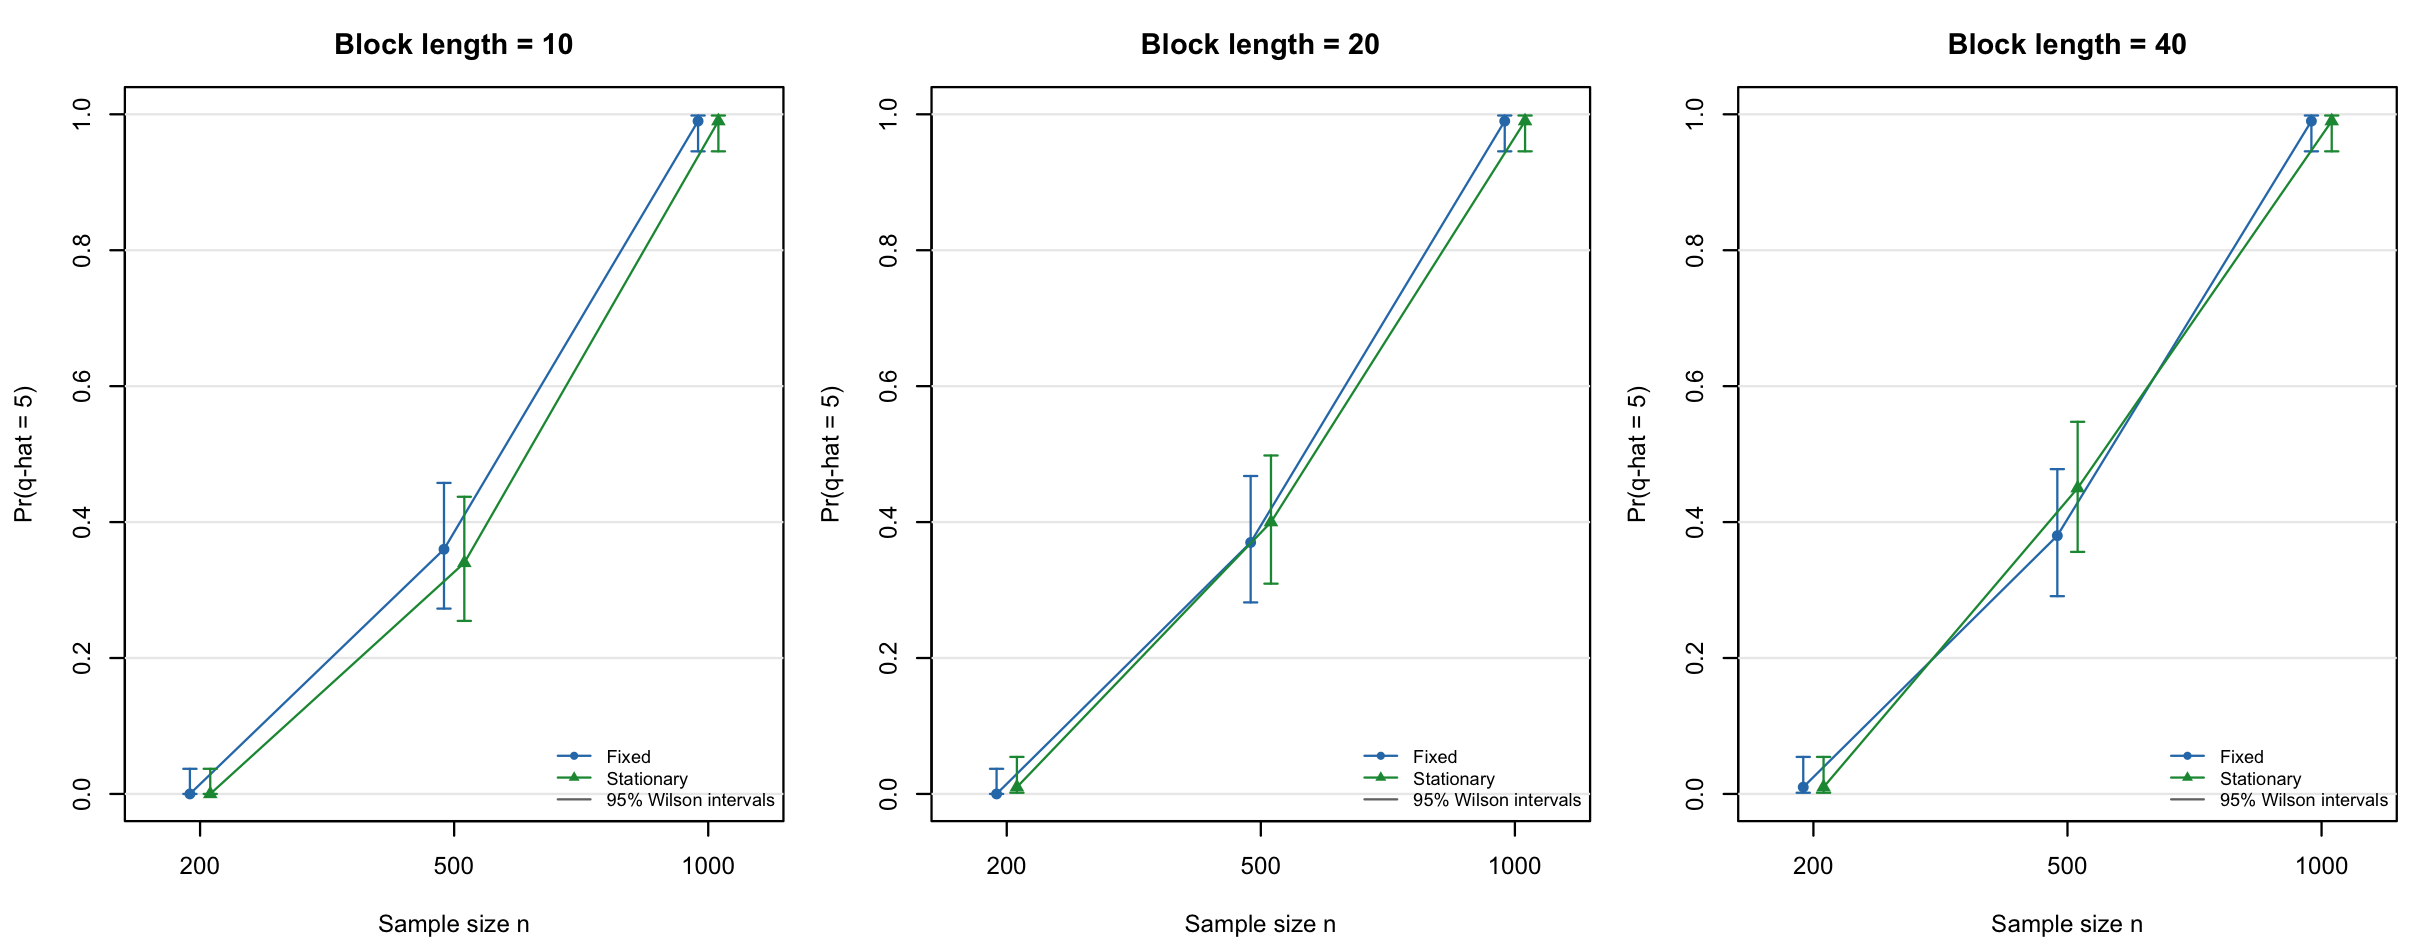
\includegraphics[width=1\textwidth,height=\textheight]{output/figures/task1_d_recovery_probability.png}

}

\caption{\label{fig-de-recovery}Correct-selection probabilities with
\(95\%\) Wilson Monte Carlo intervals. Sample sizes are displayed as
three discrete design points.}

\end{figure}

The difference between bootstrap methods is smaller than the sample-size
effect. For example, at \(n=500\) the stationary-minus-fixed differences
in recovery are \(-2\), \(3\) and \(7\) percentage points for
\(L=10,20,40\), with paired MCSEs of \(3.48\), \(3.32\) and \(3.83\)
percentage points. These standard errors are computed from the
within-dataset differences \(I_{r,S}-I_{r,F}\), accounting for the
shared datasets. The modest advantage of longer stationary blocks at
\(n=500\) should therefore not be treated as decisive evidence that one
method is universally superior. The methods give identical dimension
selections in this experiment at \(n=1000\).

\begin{figure}

{\centering 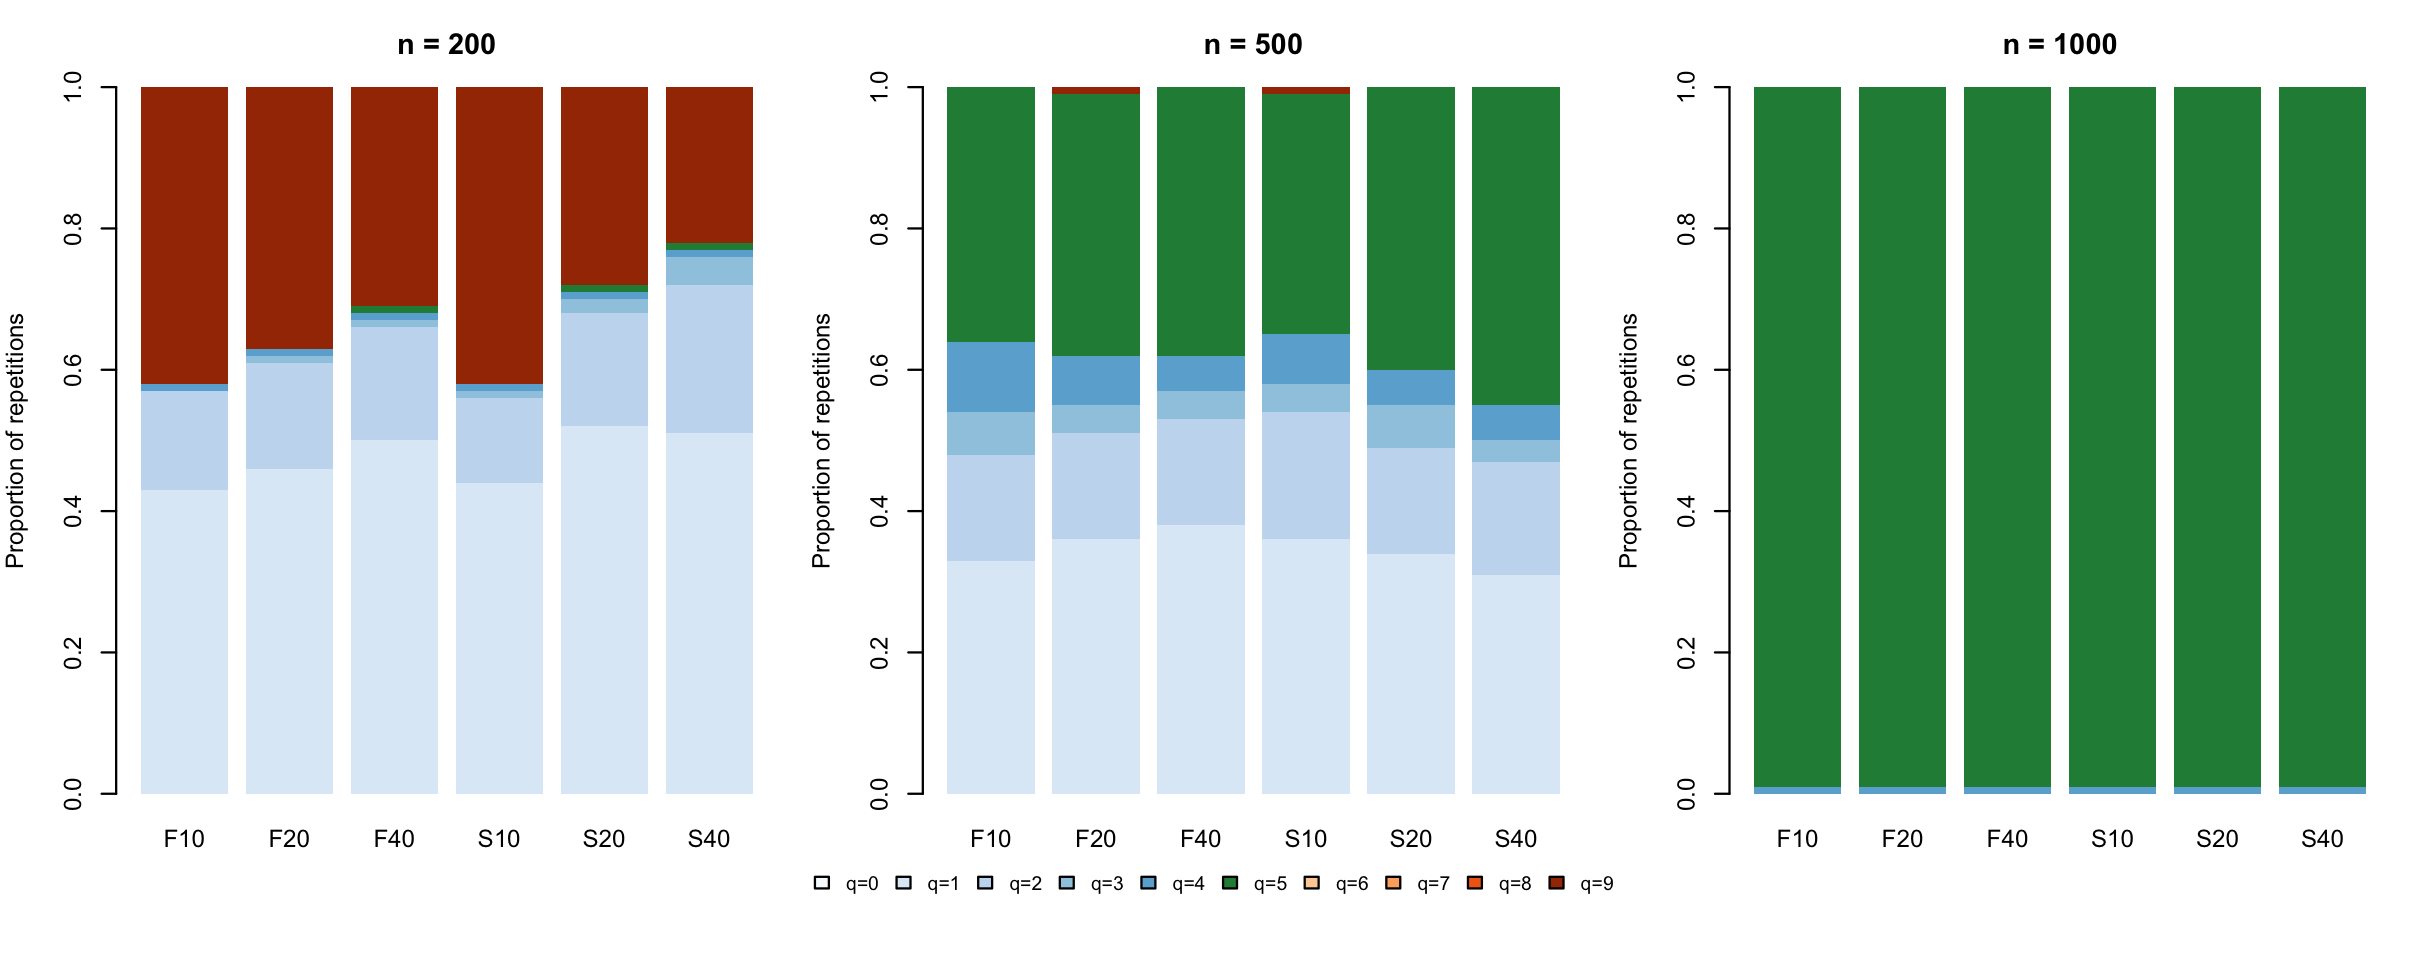
\includegraphics[width=0.95\textwidth,height=\textheight]{output/figures/task1_d_dimension_distribution.png}

}

\caption{\label{fig-de-distribution}Distribution of estimated dimensions
in Setting 1. F and S denote fixed-block and stationary bootstrap; the
number denotes \(L\). The true dimension is \(5\), shown in green.}

\end{figure}

The broad distributions for the shorter series in
Figure~\ref{fig-de-distribution} demonstrate that their poor recovery is
not merely a small bias around \(q=5\). In contrast, the long-series
distributions concentrate at the true dimension. This reproduces the
main qualitative finding of Nordhausen and Virta: SOBI-based ladle
estimation becomes reliable when the series are sufficiently long, while
short series can be inadequate. Our results provide numerical validation
under Setting 1, rather than a proof of consistency or a precise
replication of every result in the paper. They also describe the
estimator at the finite bootstrap budget \(B=100\).

\hypertarget{part-e-application-to-the-course-data}{%
\subsection{Part E: Application to the course
data}\label{part-e-application-to-the-course-data}}

\hypertarget{application-procedure-and-block-length-selection}{%
\subsubsection{Application procedure and block-length
selection}\label{application-procedure-and-block-length-selection}}

The supplied \texttt{timeseries.dat} contains \(n=1000\) observations of
\(p=10\) variables. We apply the same whitening, lag set
\(\mathcal T=\{1,\ldots,12\}\), joint diagonalization and ladle
calculations used in Part D. Both bootstrap methods are fitted at
\(L=10,20,40\). The primary choice is \(L=20\), carried forward from
Parts B--C: it permits within-block pairs at every selected lag while
retaining approximately \(50\) fixed blocks. Lengths \(10\) and \(40\)
assess how the conclusion changes when less or more temporal dependence
is preserved.

Because this application involves only one observed dataset, we increase
the bootstrap budget to \(B=500\) and repeat each method--length setting
with five independent bootstrap seeds. These \(30\) fits assess Monte
Carlo stability conditional on the same observations; they do not
constitute \(30\) independent datasets or provide a sampling confidence
interval for the true dimension. For each fit, we examine the full
curves \(f\), \(\phi\) and \(g\), the selected dimension, and the gap
between the smallest and second-smallest values of \(g\).

\hypertarget{estimated-dimension-and-supporting-evidence}{%
\subsubsection{Estimated dimension and supporting
evidence}\label{estimated-dimension-and-supporting-evidence}}

\hypertarget{tbl-de-application}{}
\begin{longtable}[]{@{}
  >{\raggedright\arraybackslash}p{(\columnwidth - 8\tabcolsep) * \real{0.1176}}
  >{\raggedleft\arraybackslash}p{(\columnwidth - 8\tabcolsep) * \real{0.0735}}
  >{\centering\arraybackslash}p{(\columnwidth - 8\tabcolsep) * \real{0.3529}}
  >{\raggedright\arraybackslash}p{(\columnwidth - 8\tabcolsep) * \real{0.2647}}
  >{\raggedleft\arraybackslash}p{(\columnwidth - 8\tabcolsep) * \real{0.1912}}@{}}
\caption{\label{tbl-de-application}Dimension estimates across five
bootstrap seeds, with \(B=500\) per fit. The last column is the smallest
gap between the two lowest criterion values across those five
runs.}\tabularnewline
\toprule\noalign{}
\begin{minipage}[b]{\linewidth}\raggedright
Method
\end{minipage} & \begin{minipage}[b]{\linewidth}\raggedleft
\(L\)
\end{minipage} & \begin{minipage}[b]{\linewidth}\centering
Observed \(\widehat q\)
\end{minipage} & \begin{minipage}[b]{\linewidth}\raggedright
Selection counts
\end{minipage} & \begin{minipage}[b]{\linewidth}\raggedleft
Minimum gap
\end{minipage} \\
\midrule\noalign{}
\endfirsthead
\toprule\noalign{}
\begin{minipage}[b]{\linewidth}\raggedright
Method
\end{minipage} & \begin{minipage}[b]{\linewidth}\raggedleft
\(L\)
\end{minipage} & \begin{minipage}[b]{\linewidth}\centering
Observed \(\widehat q\)
\end{minipage} & \begin{minipage}[b]{\linewidth}\raggedright
Selection counts
\end{minipage} & \begin{minipage}[b]{\linewidth}\raggedleft
Minimum gap
\end{minipage} \\
\midrule\noalign{}
\endhead
\bottomrule\noalign{}
\endlastfoot
Fixed & 10 & 2 & \(2\): 5 runs & 0.02019 \\
Stationary & 10 & 2 or 3 & \(2\): 4; \(3\): 1 & 0.00069 \\
Fixed & 20 & 3 & \(3\): 5 runs & 0.01278 \\
Stationary & 20 & 3 & \(3\): 5 runs & 0.02273 \\
Fixed & 40 & 3 & \(3\): 5 runs & 0.02783 \\
Stationary & 40 & 3 & \(3\): 5 runs & 0.03459 \\
\end{longtable}

Both methods consistently select \(\widehat q=3\) at \(L=20\) and
\(L=40\) (Table~\ref{tbl-de-application}). For the primary fixed-block
fit with \(L=20\) and the first seed,

\[
f(3)=0.04660,\qquad \phi(3)=0.01649,\qquad g(3)=0.06310.
\]

The next-best candidate is \(k=2\), whose criterion is larger by
\(0.01278\). The first four ordered component strengths are
approximately \(0.39989\), \(0.34474\), \(0.14143\) and \(0.03383\). The
drop after the third direction supports a three-dimensional signal
subspace, while the bootstrap component penalizes the instability
introduced by additional weak directions.

\begin{figure}

{\centering 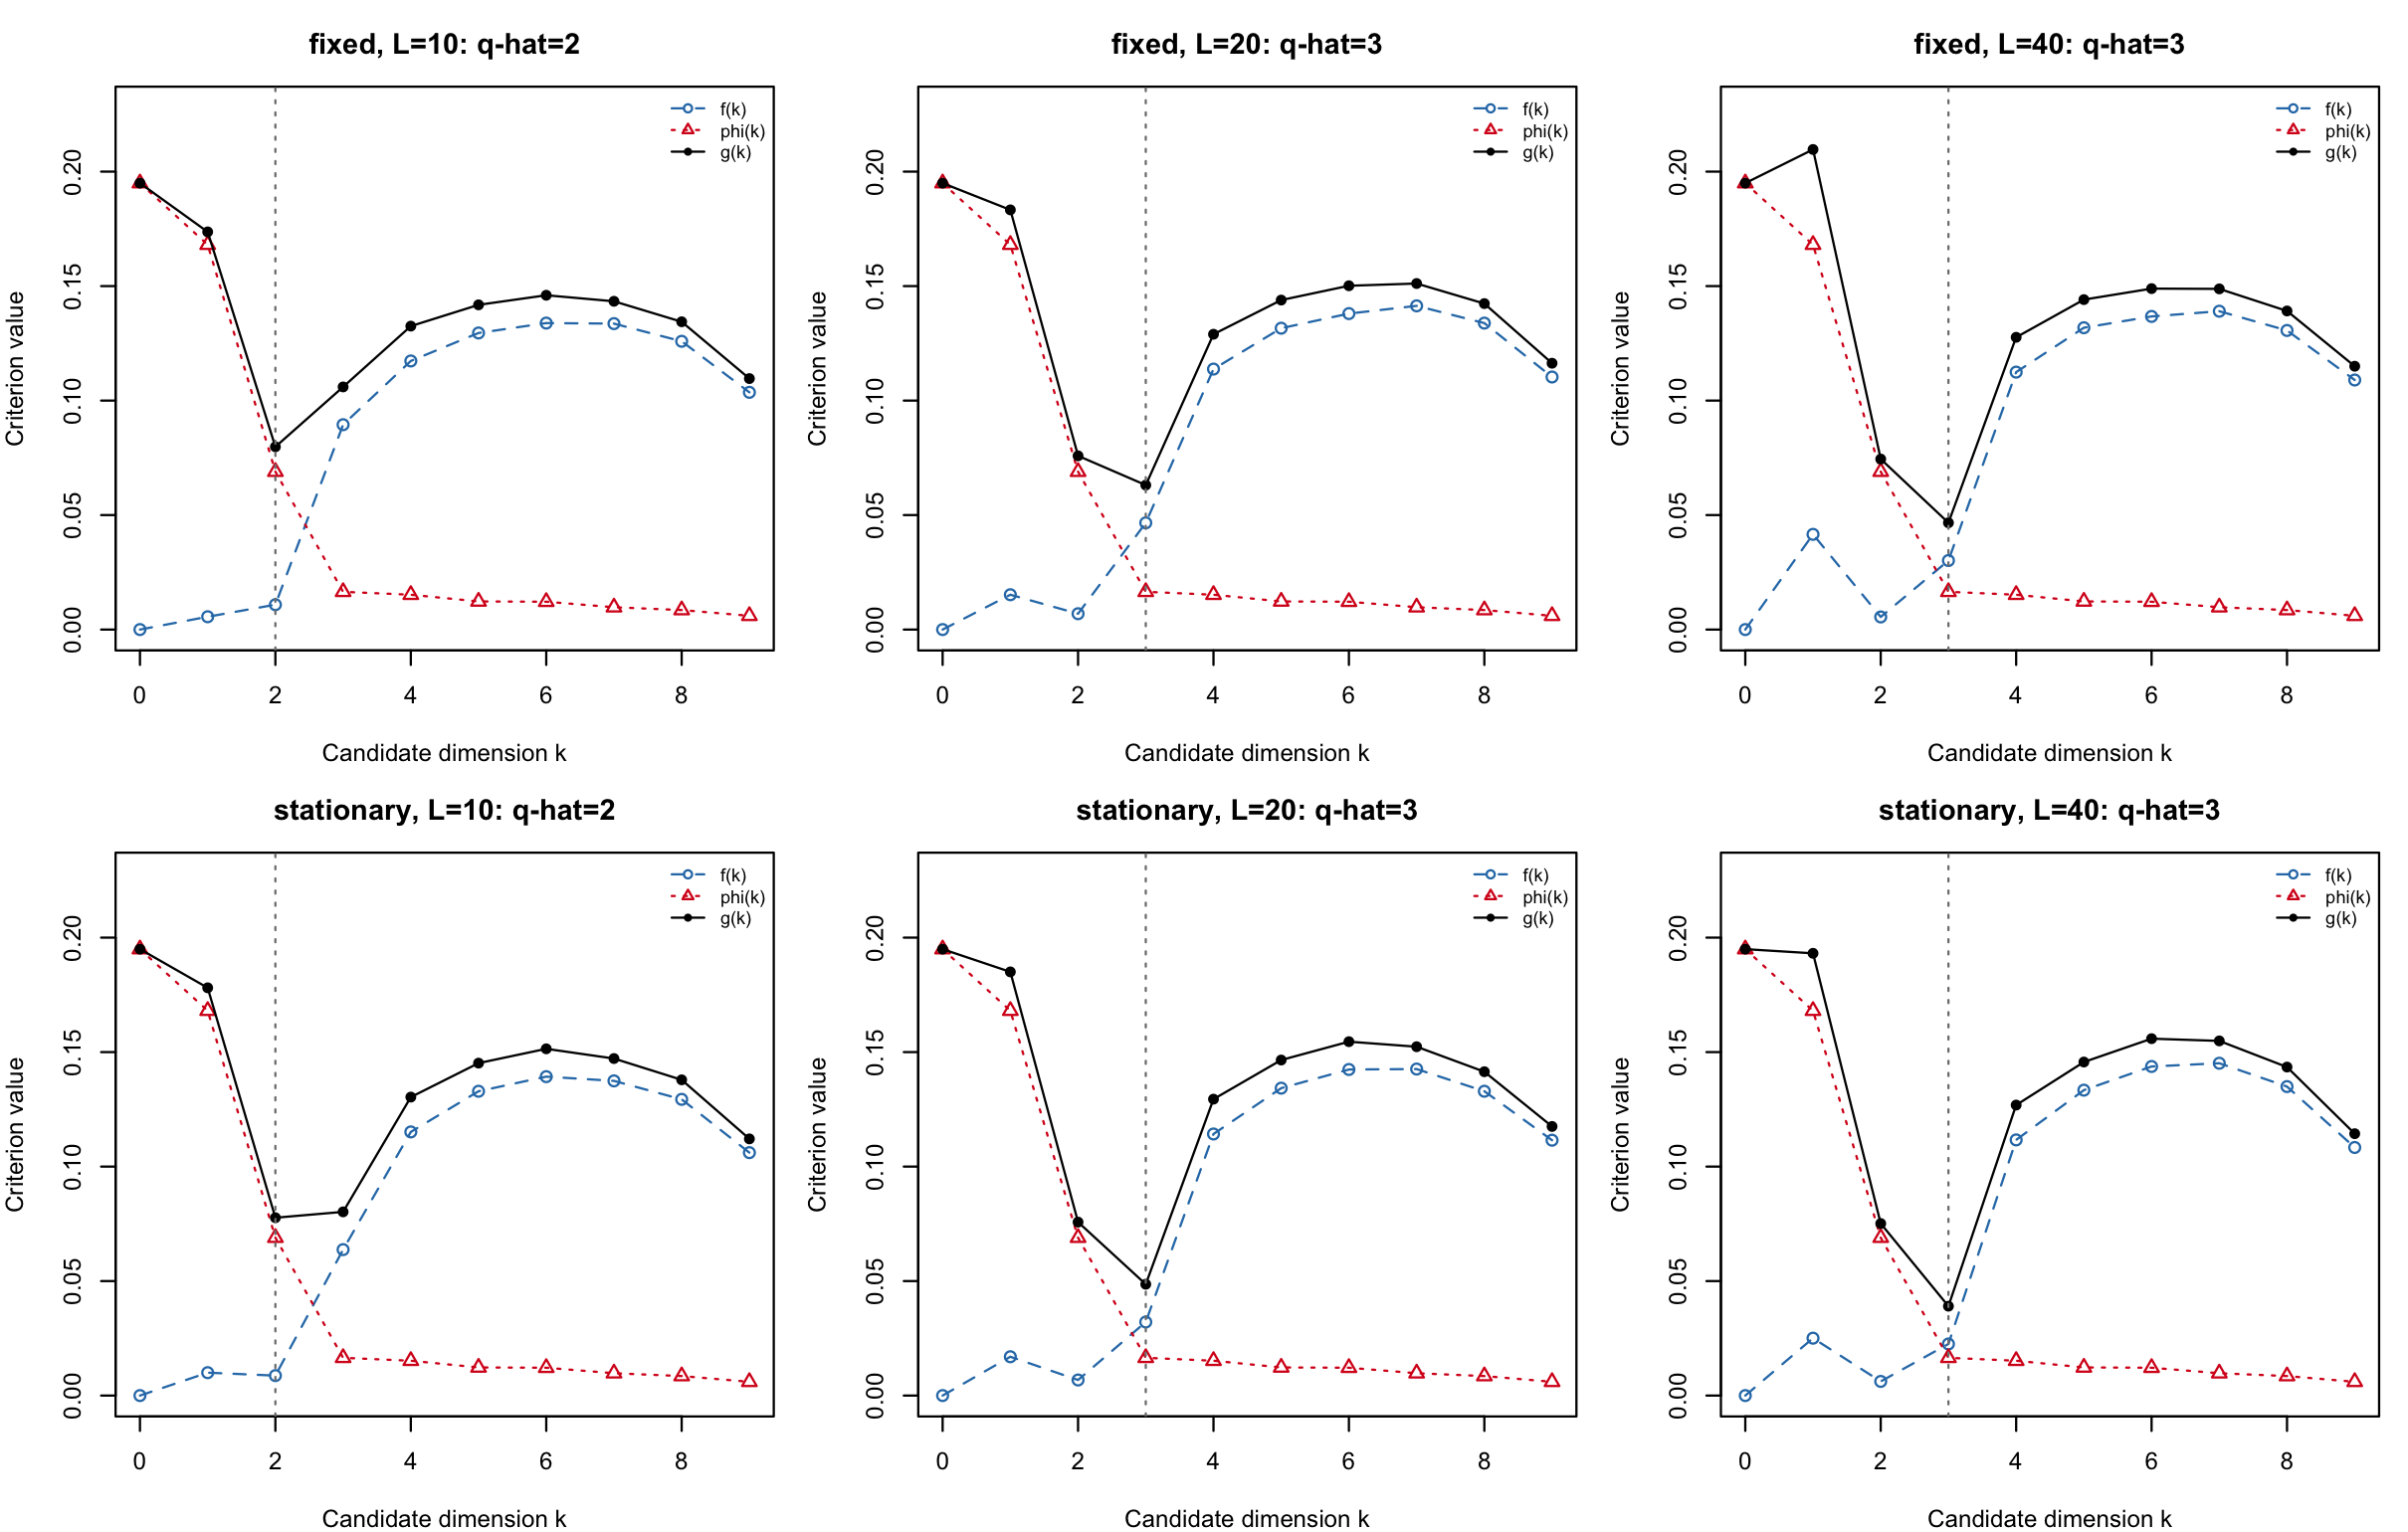
\includegraphics[width=1\textwidth,height=\textheight]{output/figures/task1_e_ladle_components.png}

}

\caption{\label{fig-de-components}Ladle components for all six settings
on the course data, using the first seed in each setting. The vertical
line marks the minimizing dimension. The value \(\phi(k)\) corresponds
to the strength of the \((k+1)\)st direction, as in Part C.}

\end{figure}

Figure~\ref{fig-de-components} shows how the two contributions determine
the minimum. The scree contribution is shared by the bootstrap settings
because it depends on the original sample, whereas \(f\) changes with
the resampling method and block length. At \(L=20\) and \(40\), the
combination has its minimum at \(3\) for both methods. However, the
results are not uniform over all block lengths: fixed blocks of length
\(10\) select \(2\) in every run, and stationary blocks with expected
length \(10\) select \(2\) in four runs and \(3\) in one. The
particularly small gap for the latter setting indicates that the two
candidates are close; it is not a hypothesis-test \(p\)-value or a
confidence level.

\hypertarget{investigating-block-length-sensitivity}{%
\subsubsection{Investigating block-length
sensitivity}\label{investigating-block-length-sensitivity}}

\begin{figure}

{\centering 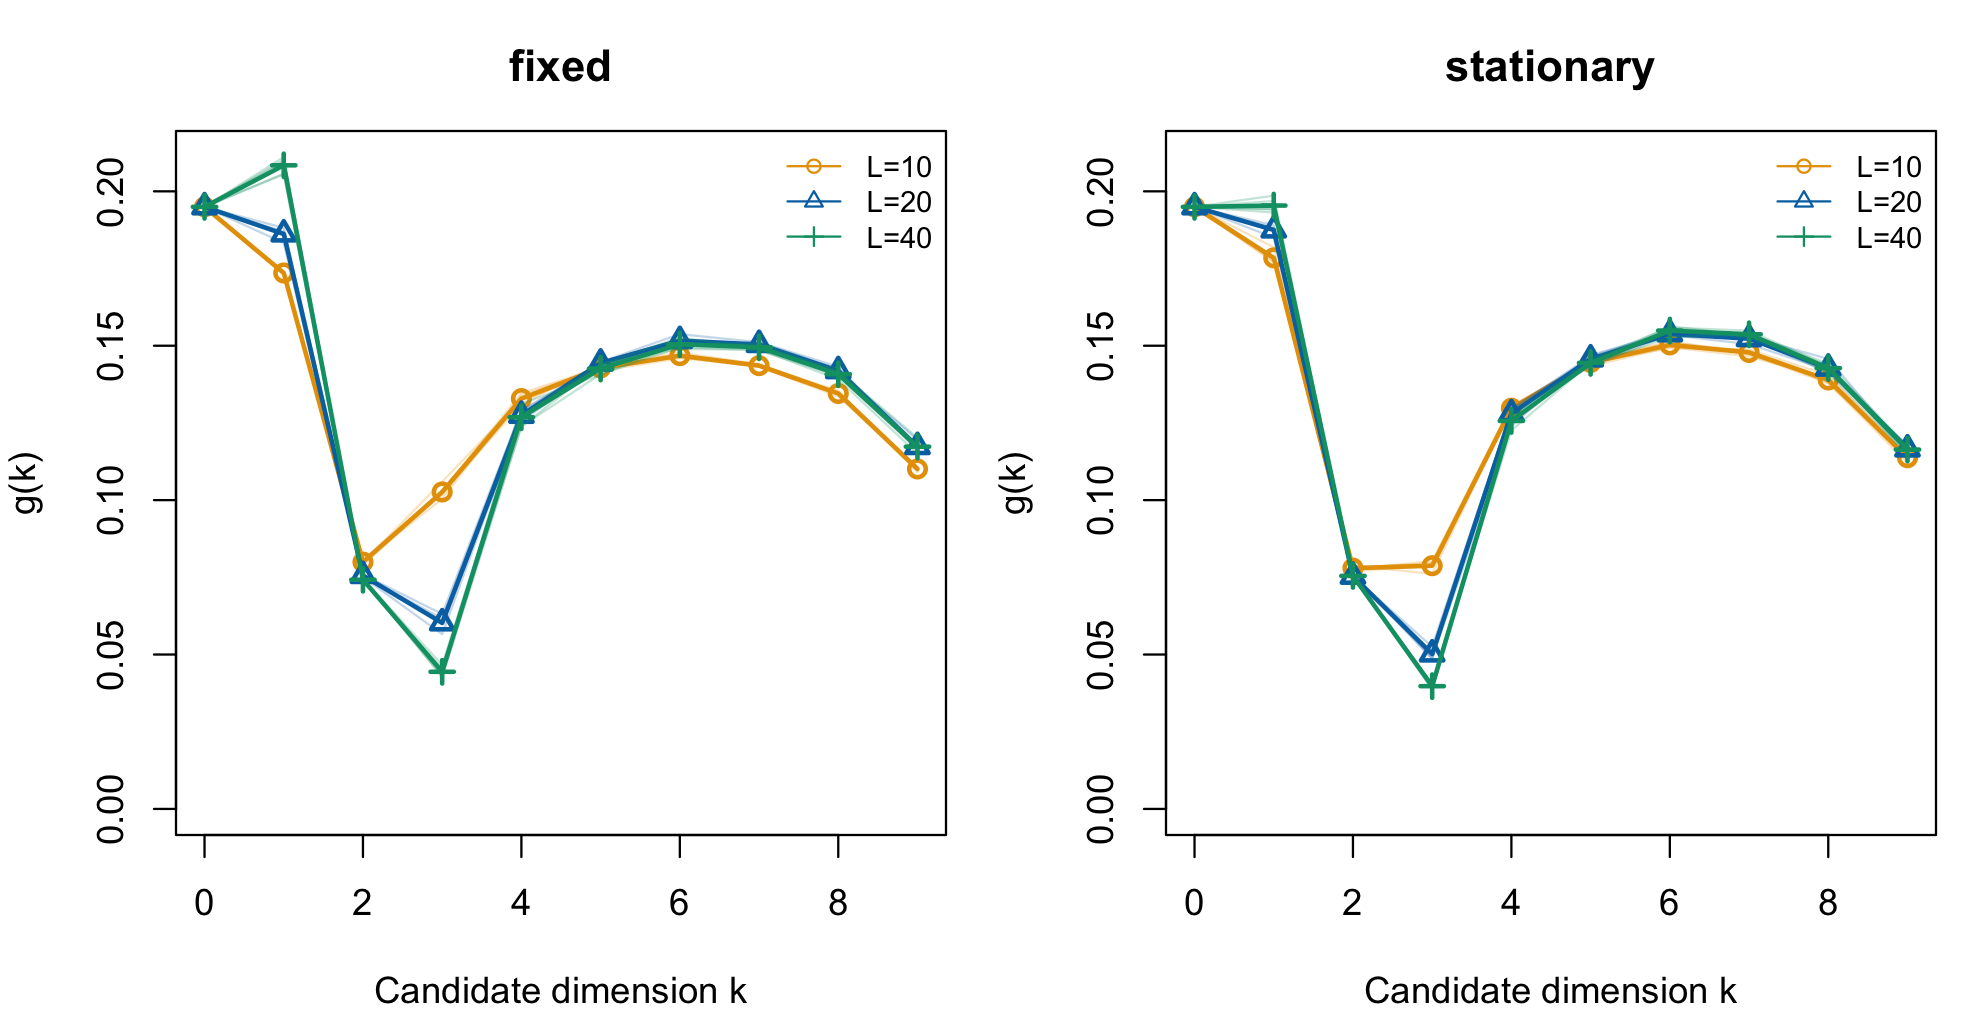
\includegraphics[width=1\textwidth,height=\textheight]{output/figures/task1_e_block_sensitivity.png}

}

\caption{\label{fig-de-sensitivity}Sensitivity of \(g(k)\) to block
length. Faint curves show the five individual seed runs; the heavier
curves show their means. The reported dimension estimates are calculated
separately for each run.}

\end{figure}

Figure~\ref{fig-de-sensitivity} shows that the main discrepancy concerns
the competition between \(k=2\) and \(k=3\). To investigate it, we
examine the ordered components obtained from the original-data
decomposition,

\[
\widehat Z=(X-\mathbf 1_n\bar x^{\mathsf T})\widehat W\widehat U.
\]

The third component has its largest absolute sample autocorrelation over
lags \(1\)--\(12\) at lag \(h=8\), where its value is approximately
\(0.287\). This relatively long-lag feature is especially vulnerable to
short blocks.

For fixed blocks, the approximate fraction of lag-\(h\) pairs lying
within one block is \(\max(1-h/L,0)\), ignoring finite-series end
effects. For stationary blocks, the probability of no restart over \(h\)
steps is \((1-1/L)^h\). At \(h=8\), these quantities are

\[
\begin{array}{c|ccc}
L & 10 & 20 & 40 \\ \hline
\text{Fixed: within-block fraction} & 0.200 & 0.600 & 0.800 \\
\text{Stationary: no-restart probability} & 0.430 & 0.663 & 0.817
\end{array}
\]

They describe preservation of local ordering, not exact autocorrelation
attenuation factors or dimension-recovery probabilities. Nevertheless,
they provide a plausible explanation for the observed sensitivity: short
blocks weaken the dependence supporting the third direction, increasing
the bootstrap instability of the three-dimensional subspace. Increasing
\(L\) makes the minimum at \(k=3\) clearer. The agreement at \(L=20\)
and \(40\), together with this dependence pattern, supports reporting
\(\widehat q=3\) as the main conclusion while explicitly retaining the
short-block alternative.

\begin{figure}

{\centering 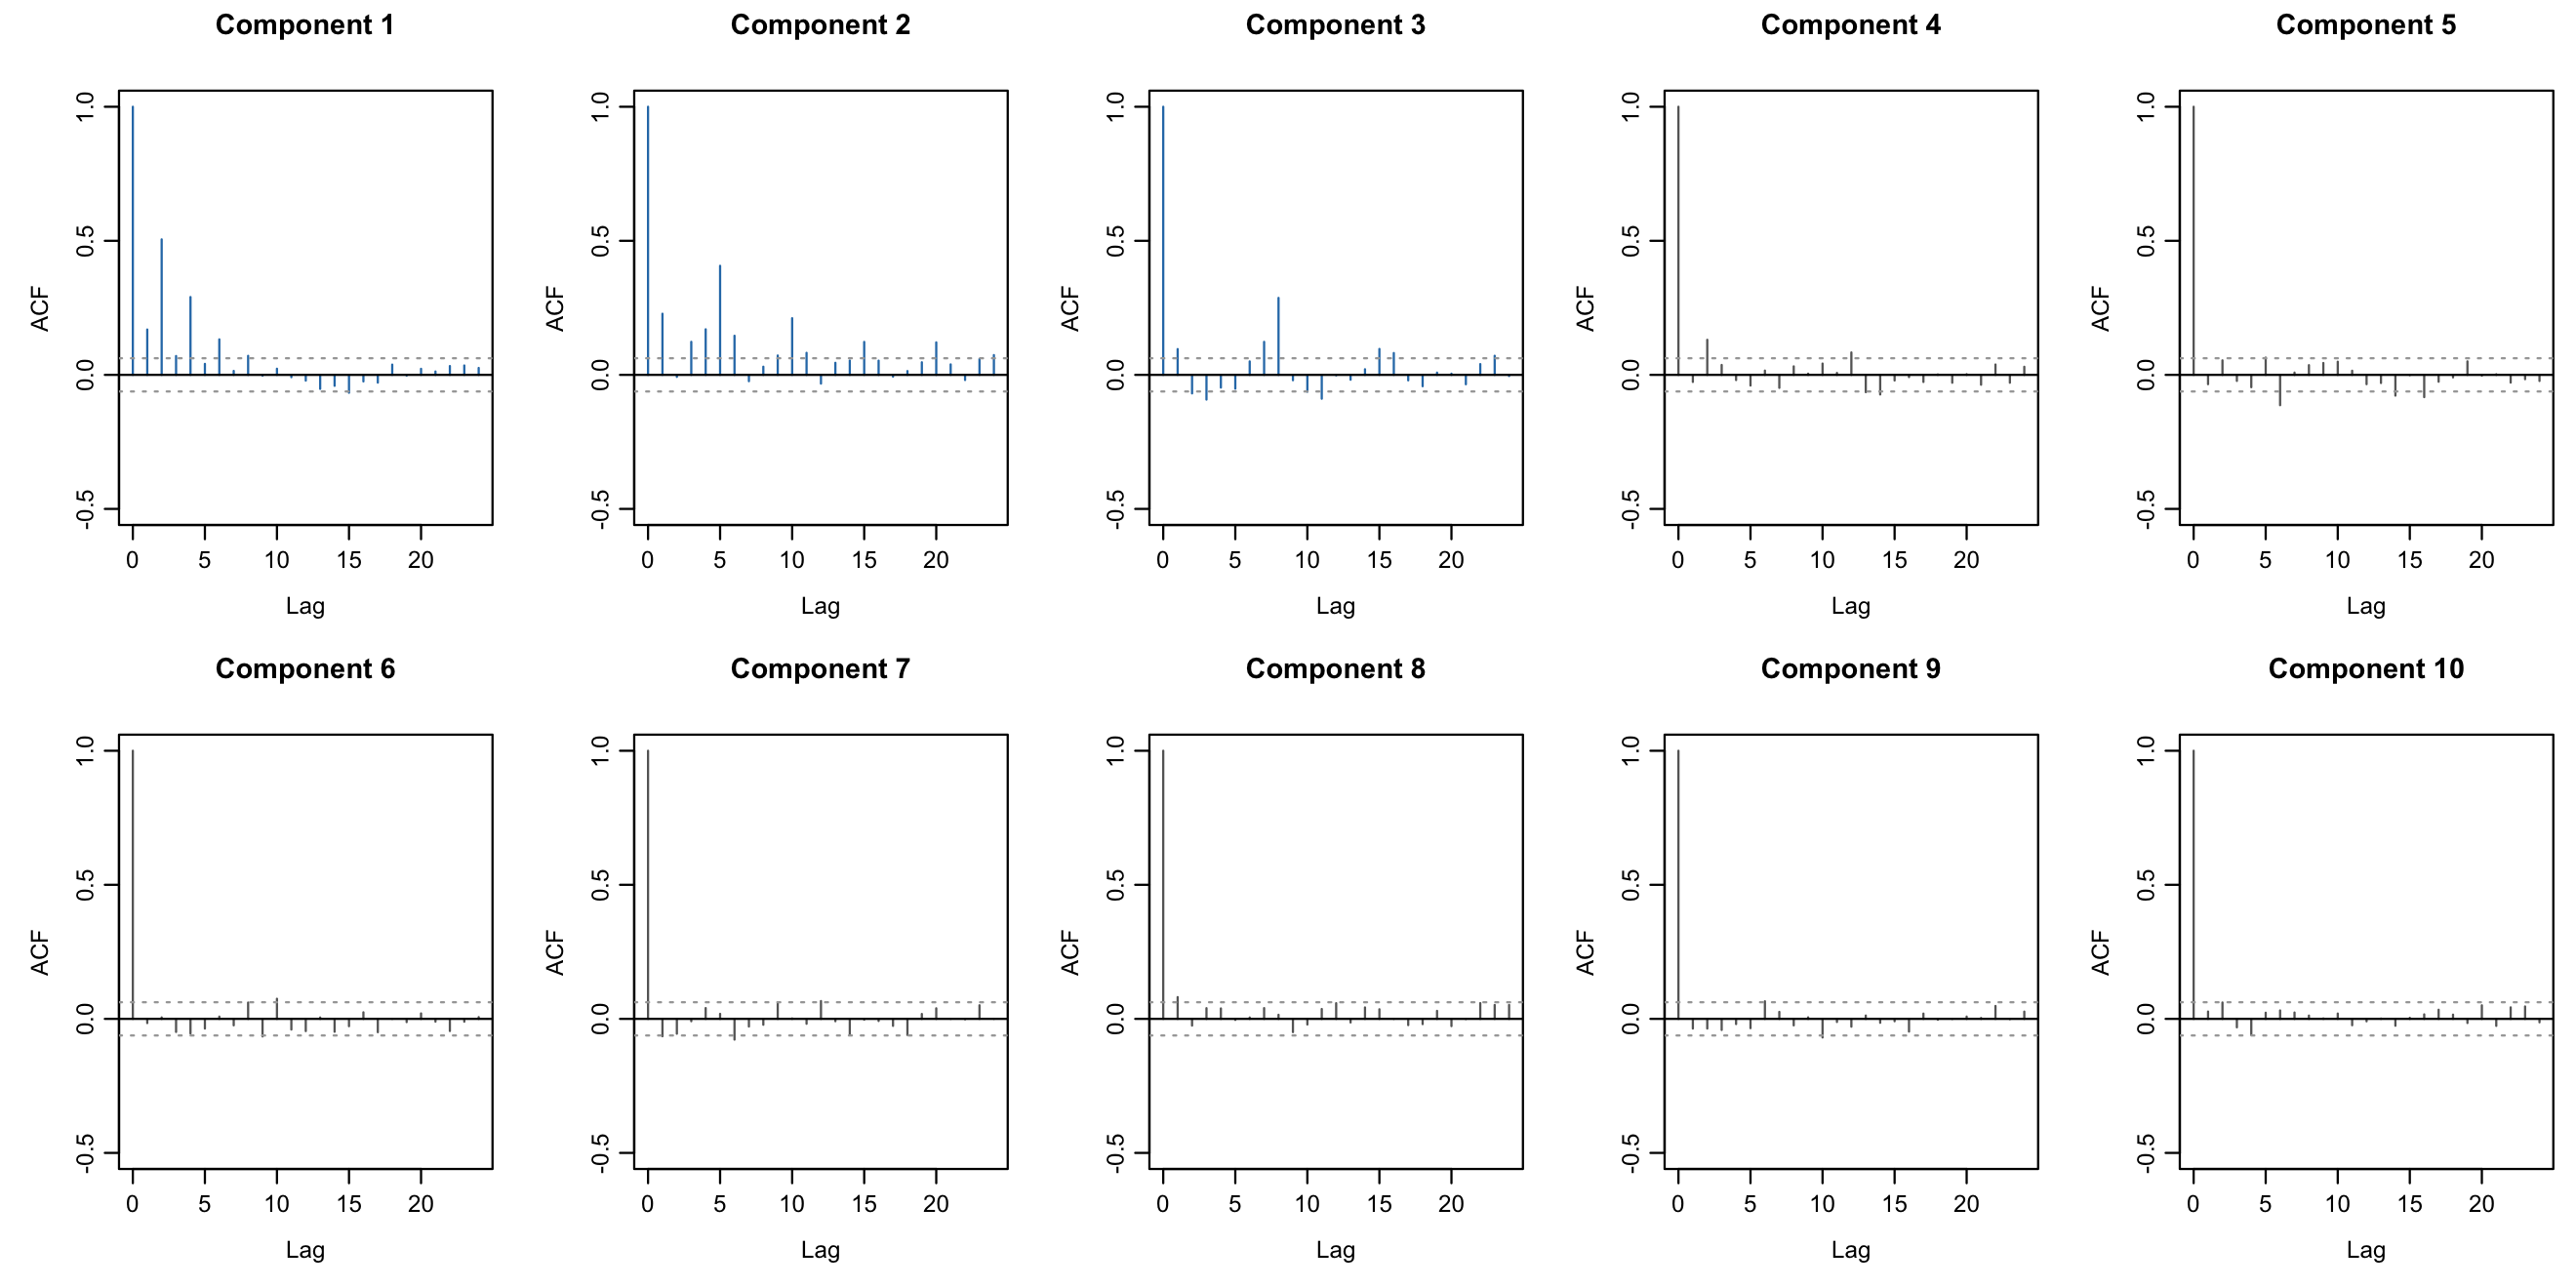
\includegraphics[width=1\textwidth,height=\textheight]{output/figures/task1_e_component_acf.png}

}

\caption{\label{fig-de-acf}Sample ACFs of the ordered components. The
first three directions, classified as signals by the primary fit, are
blue. Dashed lines at \(\pm1.96/\sqrt{1000}\) are descriptive
white-noise reference bands, not simultaneous confidence bounds after
estimating the directions.}

\end{figure}

\hypertarget{interpretation-and-limitations}{%
\subsubsection{Interpretation and
limitations}\label{interpretation-and-limitations}}

Under the second-order source-separation model, the main result suggests
three serially dependent linear combinations of the ten observed
variables and seven remaining directions with weaker dependence at the
selected lags. The first three component ACFs have pronounced features
at lags \(2\), \(5\) and \(8\), respectively (Figure~\ref{fig-de-acf}).
The remaining component strengths are smaller, although their sample
ACFs are not identically zero.

The estimated dimension counts latent linear combinations, not a subset
of three original variables. Nor does the classification establish that
the remaining directions are independent, Gaussian, or free of nonlinear
dependence. The interpretation is conditional on approximate
stationarity, the SOS model and the selected lag set. Finally,
successful recovery in Setting 1 validates the computational procedure
under that design; it does not establish the unknown dimension of this
particular dataset. Here the evidence for three directions comes from
the criterion curves, the longer-block agreement and the observed
dependence structure, with the sensitivity at \(L=10\) reported as part
of the result.

\hypertarget{task-2-bayesian-mixture-modelling-with-mcmc}{%
\section{Task 2: Bayesian mixture modelling with
MCMC}\label{task-2-bayesian-mixture-modelling-with-mcmc}}

\hypertarget{part-a-latent-variable-representation-and-gibbs-sampler}{%
\subsection{Part A: Latent-variable representation and Gibbs
sampler}\label{part-a-latent-variable-representation-and-gibbs-sampler}}

\hypertarget{part-b-simulation-study-and-computational-behaviour}{%
\subsection{Part B: Simulation study and computational
behaviour}\label{part-b-simulation-study-and-computational-behaviour}}

\hypertarget{part-c-label-switching-and-identifiability}{%
\subsection{Part C: Label switching and
identifiability}\label{part-c-label-switching-and-identifiability}}

\hypertarget{part-d-application-to-real-data}{%
\subsection{Part D: Application to real
data}\label{part-d-application-to-real-data}}



\end{document}
